\documentclass{article} % Tipo de documento

\usepackage[utf8]{inputenc} % Permite el uso de caracteres del Español

\usepackage[T1]{fontenc}

\usepackage{graphicx}

\usepackage{subfig}

% Carátula del Artículo  

\title{Reporte de Actividad 9}

\author{Brenda Leyva Amaya}

\date{28 de Abril, 2018}

\begin{document}

\maketitle % Crea el título

\begin{center}
	
\includegraphics[width=8cm]{logo.png}
\end{center}

\vspace{5.0 cm}

\section{El contexto de Maxima}

Maxima es un software libre, se puede descargar gratuitamente para varios sistemas y existe documentación extensiva que puede ser obtenida también de manera gratuita. Maxima es uno de los sistemas computacionales para álgebra  (CAS) más antiguos. Este software fue creado por el equipo de MAC en MIT en los años sesenta y fue originalmente llamado Macsyma que viene de su nombre en ingles MACs SYmbolic MAnipulator, e inicialmente se creó para las computadoras a gran escala DEC-PDP-10 que se utilizaban en esa época comunmente en las instituciones académicas. 

\vspace{0.5 cm}

En la época de los ochentas, su código se adaptó a muchas nuevas plataformas y una de sus versiones fue llamada Maxima. En 1982 MIT decide vender Macsyma como software propio y al mismo tiempo el profesor William Schelter de la Universidad de Texas continuó desarrollando la versión que se había denominado Maxima. A finales de los ochentas aparecieron algunos otros sistemas similares a Macsyma como Maple y Mathematica. En 1998, el profesor Schelter obtuvo autorización del Departamento de energía (DOE) para distribuir el código fuente de Maxima como software libre. 

\vspace{0.5 cm}

Existen variadas interfaces para trabajar con Maxima, se puede accesar corriendo un comando shell o directamente en una interface gráfica como wxMaxima, imaxima o Xmaxima. 

\begin{center}

	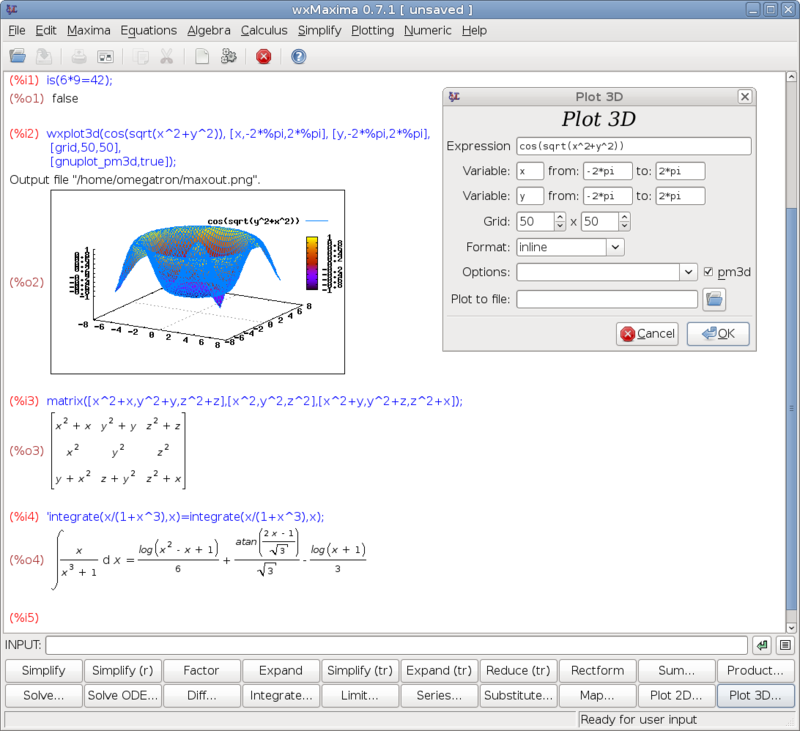
\includegraphics[width=9cm]{WxMaxima.png}
    
    Aspecto de Maxima y experiencia de usuario en wxMaxima.
    
\end{center}

\section{Principales funciones y comandos}

A continuación se presentan las principales funciones de Maxima y los comandos respectivos, así como ejemplos de su uso. 

\subsection{Entrada y salida de datos}

Cuando una sesión de Maxima comienza, aparece la etiqueta i1, esto indica que se trata de la primer entrada, "Entrada 1". Un comando válido debe ser escrito justo después de esta etiqueta., finalizada con un punto y coma, cuando se utiliza la combinación de teclas shift+enter esta entrada será procesada y simplificada, se ligará a una variable interna. i1 y su resultado serán mostrados seguidos por la tique "o1" la cual significa "salida 1", este resultado también será ligado a una variable interna. A continuación una nueva etiqueta aparecerá en pantalla i2, lo cual indica que se puede colocar una nueva entrada, "Entrada 2". 

\vspace{0.5 cm}

Se deben tomar en cuenta dos aspectos muy importantes de Maxima. El primero es que existen ciertos comandos como log(2) en los cuales maxima no podrá mostrar el resultado pues se trata de un numero irracional que no puede ser representado como un número finito con una cierta cantidad de números. El segundo es que el símbolo "*" siempre deberá incluirse en los productos, además de paréntesis siempre que se trate del argumento de una función. Maxima podrá proporcionar información de cualquier función, solo es necesario realizar un comando de la siguiente manera: "? funcion". En maxima al terminar una entrada con un signo de dólar se lleva a cabo el comando pero no nos muestra el resultado en pantalla. 

\subsection{Números}

Maxima acepta números reales y complejos. Los números reales en maxima pueden ser enteros, racional o de punto flotante, los números irracionales como lo es raíz de 2 o logaritmo de 2 permaneces en esa forma (solo expresados). Los resultados de operaciones hechas con números en formato de punto flotante se presentarán también en este formato. 

\vspace{0.5 cm}

Al trabajar con maxima para evitar errores relacionados al uso de números de punto flotante, es recomendable utilizar en su lugar fracciones, por ejemplo se tendría 1/10 en lugar de 0.1. Sin embargo existe otro formato en maxima que acepta cualquier número racional cuando es representado en número flotante, este formato se llama "big float" y se indica su uso con la letra "b" en el lugar de la usual "e" para los exponentes, por ejemplo 2.56x1020 que se escribiría como 2.56e20 se representaría internamente con precisión doble, pero si el mismo número se indica como 2.56b20, se representará internamente como un "big float" con una mayor cantidad de dígitos considerados al operar. La función "bfloat" convierte un número a formato big float. Una letra b seguida de un cero al final de un resultado significa que el núemro está en el formato de big float y que necesitará ser multiplicado por un factor de 100=1. 

\subsection{Variables}

Para ligar un valor u otros objetos a una variable se utiliza el símbolo ":" y no es signo de igual "=" pues este se utilizará para definir ecuaciones matemáticas. El nombre de las variables puede ser cualquier combinación de letras, número y alguno de los símbolos de por ciento y guión bajo, sin embargo el primer caracter no puede ser un número y se deberá considerar que maxima es sensible a las letras minúsculas y mayúsculas. 

\vspace{0.5 cm}

Se puede remover el valor ligado a una variable, esto con la función "remvalue" para una variable en específico o "remvalue (all)" para todas. Es bueno notar que una variable se puede ligar a un valor numérico, a una expresión algebraica o a cualquier otro objeto de maxima. Para sustituir una variable en una expresión por un valor se utiliza el comando "subst". Es recomendable al manipular variables no utilizar nombres que ya se estén utilizando por "default" en maxima. Otro aspecto importante es que maxima simplifica internamente la mayoría de las entradas antes de ejecutarlas. 

\subsection{Listas}

Una variable también se puede ligar a una lista de valores, estos se indican entre corchetes y se separan por comas. Muchas de las operaciones que se realizan en maxima entre números, también se puede realizar entre listas. Los elementos de una lista son etiquetados por números enteros comenzando por el 1. Para referenciar sólo un elemento de la lista se escribe el índice correspondiente entre corchetes. 

\vspace{0.5 cm}

Una función muy útil para crear listas es "makelist", esta expande una expresión, reemplaza varios valores distintos por alguna variable. El primer argumento que se le indica a makelist debe ser la expresión a expandir y el segundo argumento es el nombre de la variable que será reemplazada por una secuencia de valores, un valor inicial y hasta uno máximo definido por el tercer y cuarto argumento. Si se proporciona un quinto elemento será utilizado como el incremento en la secuencia de valores que se reemplazarán, en caso de no indicarlo, el incremento default es de 1. 


\subsection{Constantes}

Maxima contiene algunas constantes matemáticas predefinidas. Los nombres de las variables ligadas a esas constantes casi siempre comienzan con el signo de por ciento. Tres constantes importantes o principales son pi, el número de Euler, la base natural de los logaritmos (e) y el número imaginario i. 

\subsection{Archivos de comando}

Para guardar todos los comandos que se han insertado durante una sesión de trabajo en maxima, existe la opción "Save Maxima Input to File" en el menú "File". El archivo creado con esta opción se puede accesar más tarde en una nueva sesión. En este caso se pueden correr todos los comandos contenidos en la sesión con "Batch file" en el mismo menú "File".

\vspace{0.5 cm}

Se pueden agregar comentarios a estos archivos comenzando con los símbolos /* y terminando con */. Una manera eficiente de trabajar con maxima consiste en comenzar un archivo para escritura llamado "batch" con los comandos que se utilizarán, este después se podrá descargar con la opción "Batch file". De esta manera si aparece un error se vuelve innecesario volver a ingresar los comandos, será suficiente con corregir el comando en el archivo previo y volver a descargarlo en maxima. 

\subsection{Álgebra}

Las expresiones pueden incluir operaciones matemáticas con variables abstractas. Estas expresiones pueden ser manipuladas y producir expresiones nuevas a raíz de ellas. El signo de igual se utiliza para definir ecuaciones matemáticas. 


\vspace{0.5 cm}

Para encontrar las raíces de un polinomio se utiliza la función "allroots". Para resolver un sistema de ecuaciones, el cual puede ser lineal o no lineal, el primer argumento que se proporciona es la lista con las ecuaciones y el segundo argumento deberá ser otra lista con los nombres de las variables. Adempás de estos ejemplos mencionados, maxima cuenta con una enorme variedad de alternativas de manejo algebraico que se seguirán empleando en el futuro. 

\subsection{Trigonometría}

En lo que respecta a trigonometría maxima funciona con una sintaxis similar a la de cualquier lenguaje computacional, se tiene la funcion seguida de la variable o el valor del ángulo entre paréntesis. 

\subsection{Cálculo}

Maxima tiene herramientas de diferenciación e integración, tanto sencillas como múltiples, así como diferenciación e integración parcial e implícita. 

\subsection{Funciones}

Las funciones en maxima son análogas a las funciones en programación es una acción que es llamada y seguida del valor que se ingresa entre parentésis. A la función se le alimenta este cierto valor y esta nos proporciona un resultado conforme al algoritmo correspondiente. 

\subsection{Graficación}

Maxima nos permite realizar graficación en 3d y 2d, estas funciones se accesan en el módulo de graficación aceptando tanto funciones implícitas como parametrizaciones. Las herramientas de graficación en wxmaxima son altamente intuitivas y por lo tanto la experiencia de usuario es muy buena. Vease aquí abajo la pantalla que muestra las opciones de graficación 3D como ejemplo:

\begin{center}

	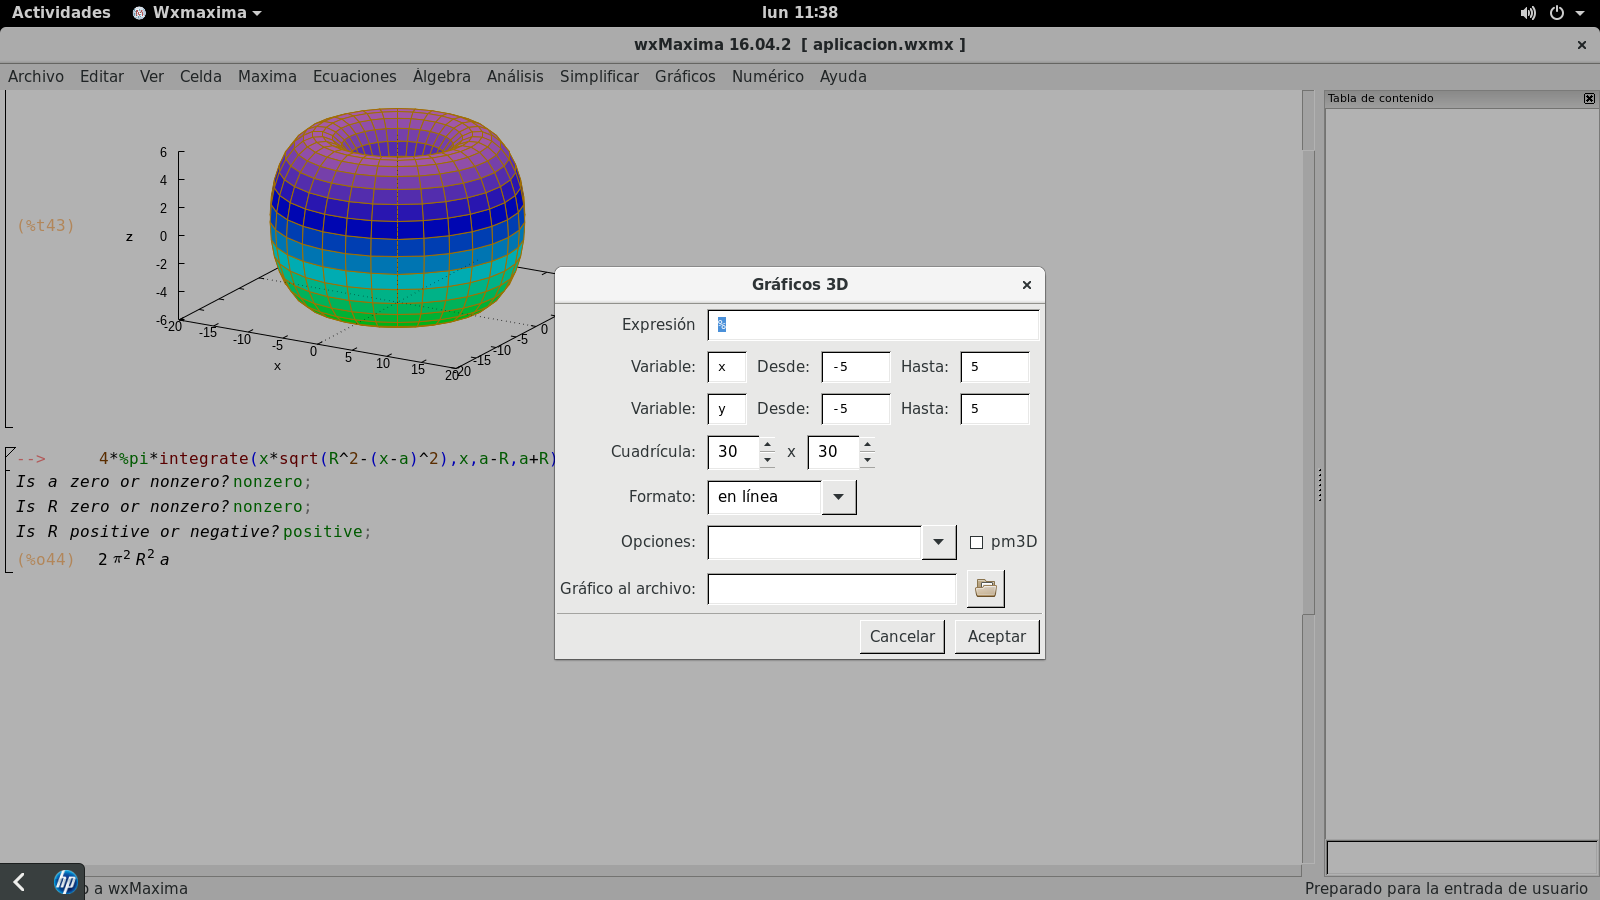
\includegraphics[width=10cm]{pantalla.png}
    
    Herramienta de graficación 3D.
    
\end{center}


\section{Un problema a resolver}

Para utilizar las herramientas disponibles en maxima se planteará el problema de encontrar el volúmen y la gráfica correspondiente a un toroide. La integral se plantea como sigue:

\begin{verbatim} 

4*%pi*integrate(x*sqrt(R^2-(x-a)^2),x,a-R,a+R);

"Is "a" zero or nonzero?"  nonzero;
"Is "R" zero or nonzero?"  nonzero;
"Is "R" positive or negative?"  positive;

RESULTADO:  2*%pi^2*R^2*a

\end{verbatim}

** A continuación la gráfica correspondiente:

\begin{center}

	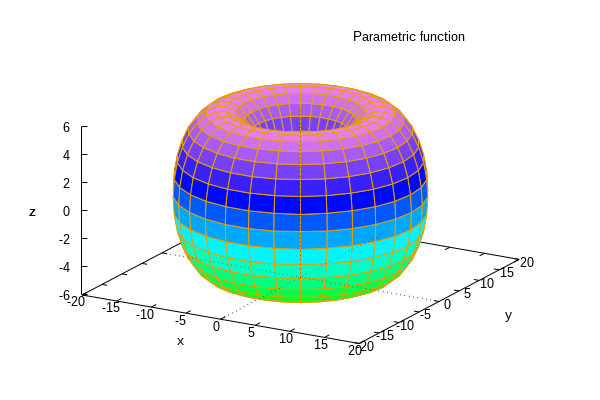
\includegraphics[width=9cm]{toroide.png}
    
\end{center}




\section*{Bibliografía y fuentes}

\begin{verbatim} 
Maxima (software). (2018, April 10). 
Retrieved from https://en.wikipedia.org/wiki/Maxima_(software) 
\end{verbatim}


\begin{verbatim} 
(n.d.). Retrieved from https://def.fe.up.pt/dynamics/maxima_tutorial.html
\end{verbatim}


\begin{verbatim} 
http://euler.us.es/~renato/clases/maxima/manualesPDF/maxima-manual-UGR.pdf
\end{verbatim}



\section*{Apéndice}

\hspace{0.5 cm} ¿Cuál fue tu primera impresión de wxmaxima?

\vspace{0.5 cm}

** Maxima es una herramienta muy útil y parece ser sencilla de usar.

\vspace{0.5 cm}

¿Crees que esta herramienta puede ser útil en otros de tus cursos?

\vspace{0.5 cm}

** Si, considero que seguirá siento útil en todas las áreas de aplicación de la licenciatura.

\vspace{0.5 cm}
 
 ¿Qué se te dificultó mas en esta actividad?
 
\vspace{0.5 cm}

** Realizar la síntesis de ideas principales y herramientas principales.

\vspace{0.5 cm}

¿Se te hizo compleja esta actividad? ¿Cómo la mejorarías? 

\vspace{0.5 cm}

** No, no me pareció compleja. Me parecería bien el incluir un ejemplo ya realizado en el cual se utilicen muchas de las herramientas que tiene wxmaxima y así poder observar sus posibilidades desde un primer acercamiento. 




\end{document}